% !TeX root = ../SPL-Rules.tex
% !TeX spellcheck = en_US
\section{Setup of the Environment}
\label{sec:setup_environment}

\subsection{Field Construction}
\label{sec:field_dim}

The standard soccer field consists of \qty{8}{\milli\metre} artificial turf mounted on a flat wooden base with a total area of length~\qty{\TotalLength}{\metre} and width~\qty{\TotalWidth}{\metre}. Care should be taken to ensure the field is as flat and level as possible. Additionally, the wooden base should be well-supported and should not give when humans stand or walk on it.

\Cref{fig:field_dim} shows the dimensions of a standard soccer field.
A more detailed technical drawing is provided in \cref{apx:technical-drawing} to this document.
Note that the penalty cross is a cross and there is a dash at center field. White field lines can be made of the same \qty{8}{\milli\metre} artificial turf, but in white (\ie, made of white artificial turf), spray-painted or taped. Regardless of the solution, the field lines must be durable throughout the competition.

\Cref{fig:goal_dimensions} and \cref{fig:goal_appearance} depict the construction and placement of the goals. A support structure for the net shall be made with small black, white, or gray bars or cylinders.  The support structure shall be constructed exactly as shown in \cref{fig:goal_appearance}.

\begin{figure}[b!]
\centering
\centerline{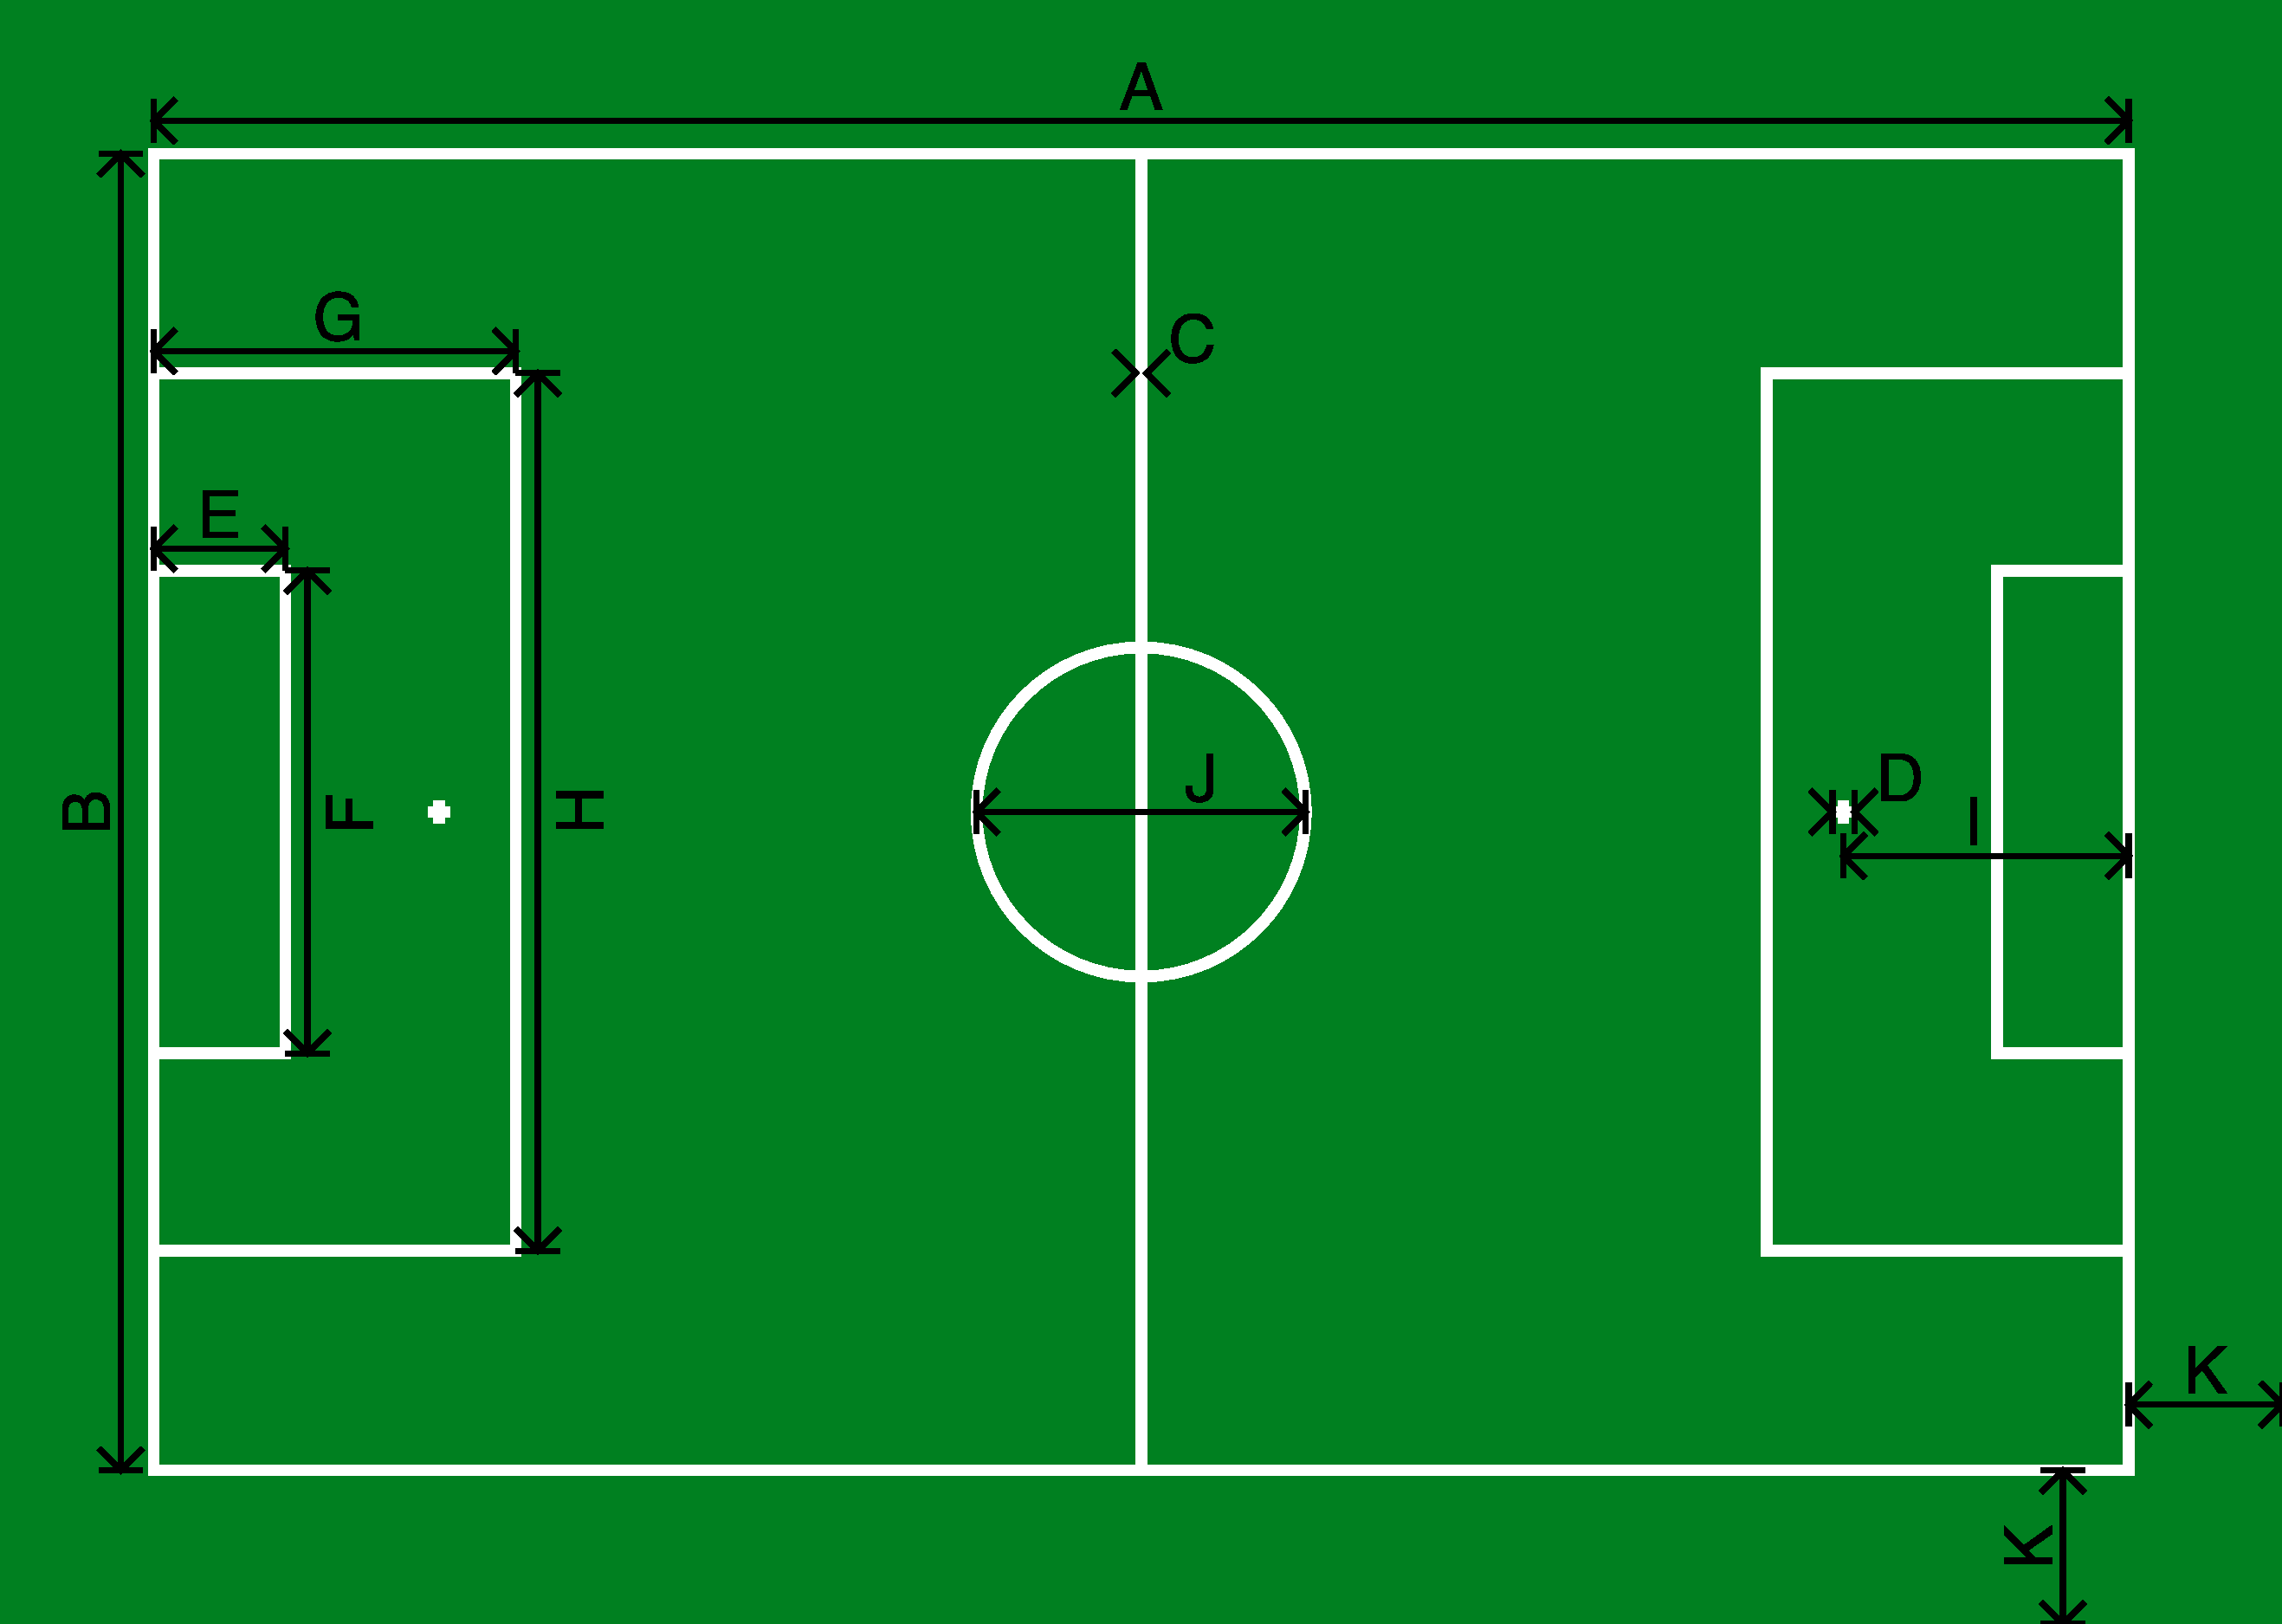
\includegraphics[width=\columnwidth]{figs/fieldDimensions2020.pdf}}
\vspace{1ex}
\begin{tabular}{| l | l | l |}
ID & Description & Length (in mm) \\
\hline \hline
A & Field length & 9000 \\
\hline
B & Field width & 6000 \\
\hline
C & Line width & 50 \\
\hline
D & Penalty cross size & 100 \\
\hline
E & Goal area length & 600 \\
\hline
F & Goal area width & 2200 \\
\end{tabular}
\begin{tabular}{|l|l|l|}
ID & Description & Length (in mm) \\
\hline \hline
G & Penalty area length & 1650 \\
\hline
H & Penalty area width & 4000 \\
\hline
I & Penalty cross distance & 1300 \\
\hline
J & Center circle diameter & 1500 \\
\hline
K & Border strip width & 700 \\
\hline
 &  &  \\
\end{tabular}
\caption{Schematic diagram of the soccer field (not to scale) and corresponding dimensions in mm.  Note that measurements on this diagram are made to the center of lines.}
\label{fig:field_dim}
\end{figure}


\begin{figure}[t!]
\begin{center}
\leavevmode
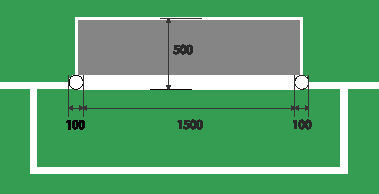
\includegraphics[width=1\columnwidth]{figs/goalDimensions2015.pdf}
\caption{Dimensions of the goal (in mm), viewed from above, and its placement on the field.}
\label{fig:goal_dimensions}
\end{center}
\end{figure}

\begin{figure}[h!]
\begin{center}
\leavevmode
\begin{minipage}[t]{0.49\columnwidth}
\imagebox{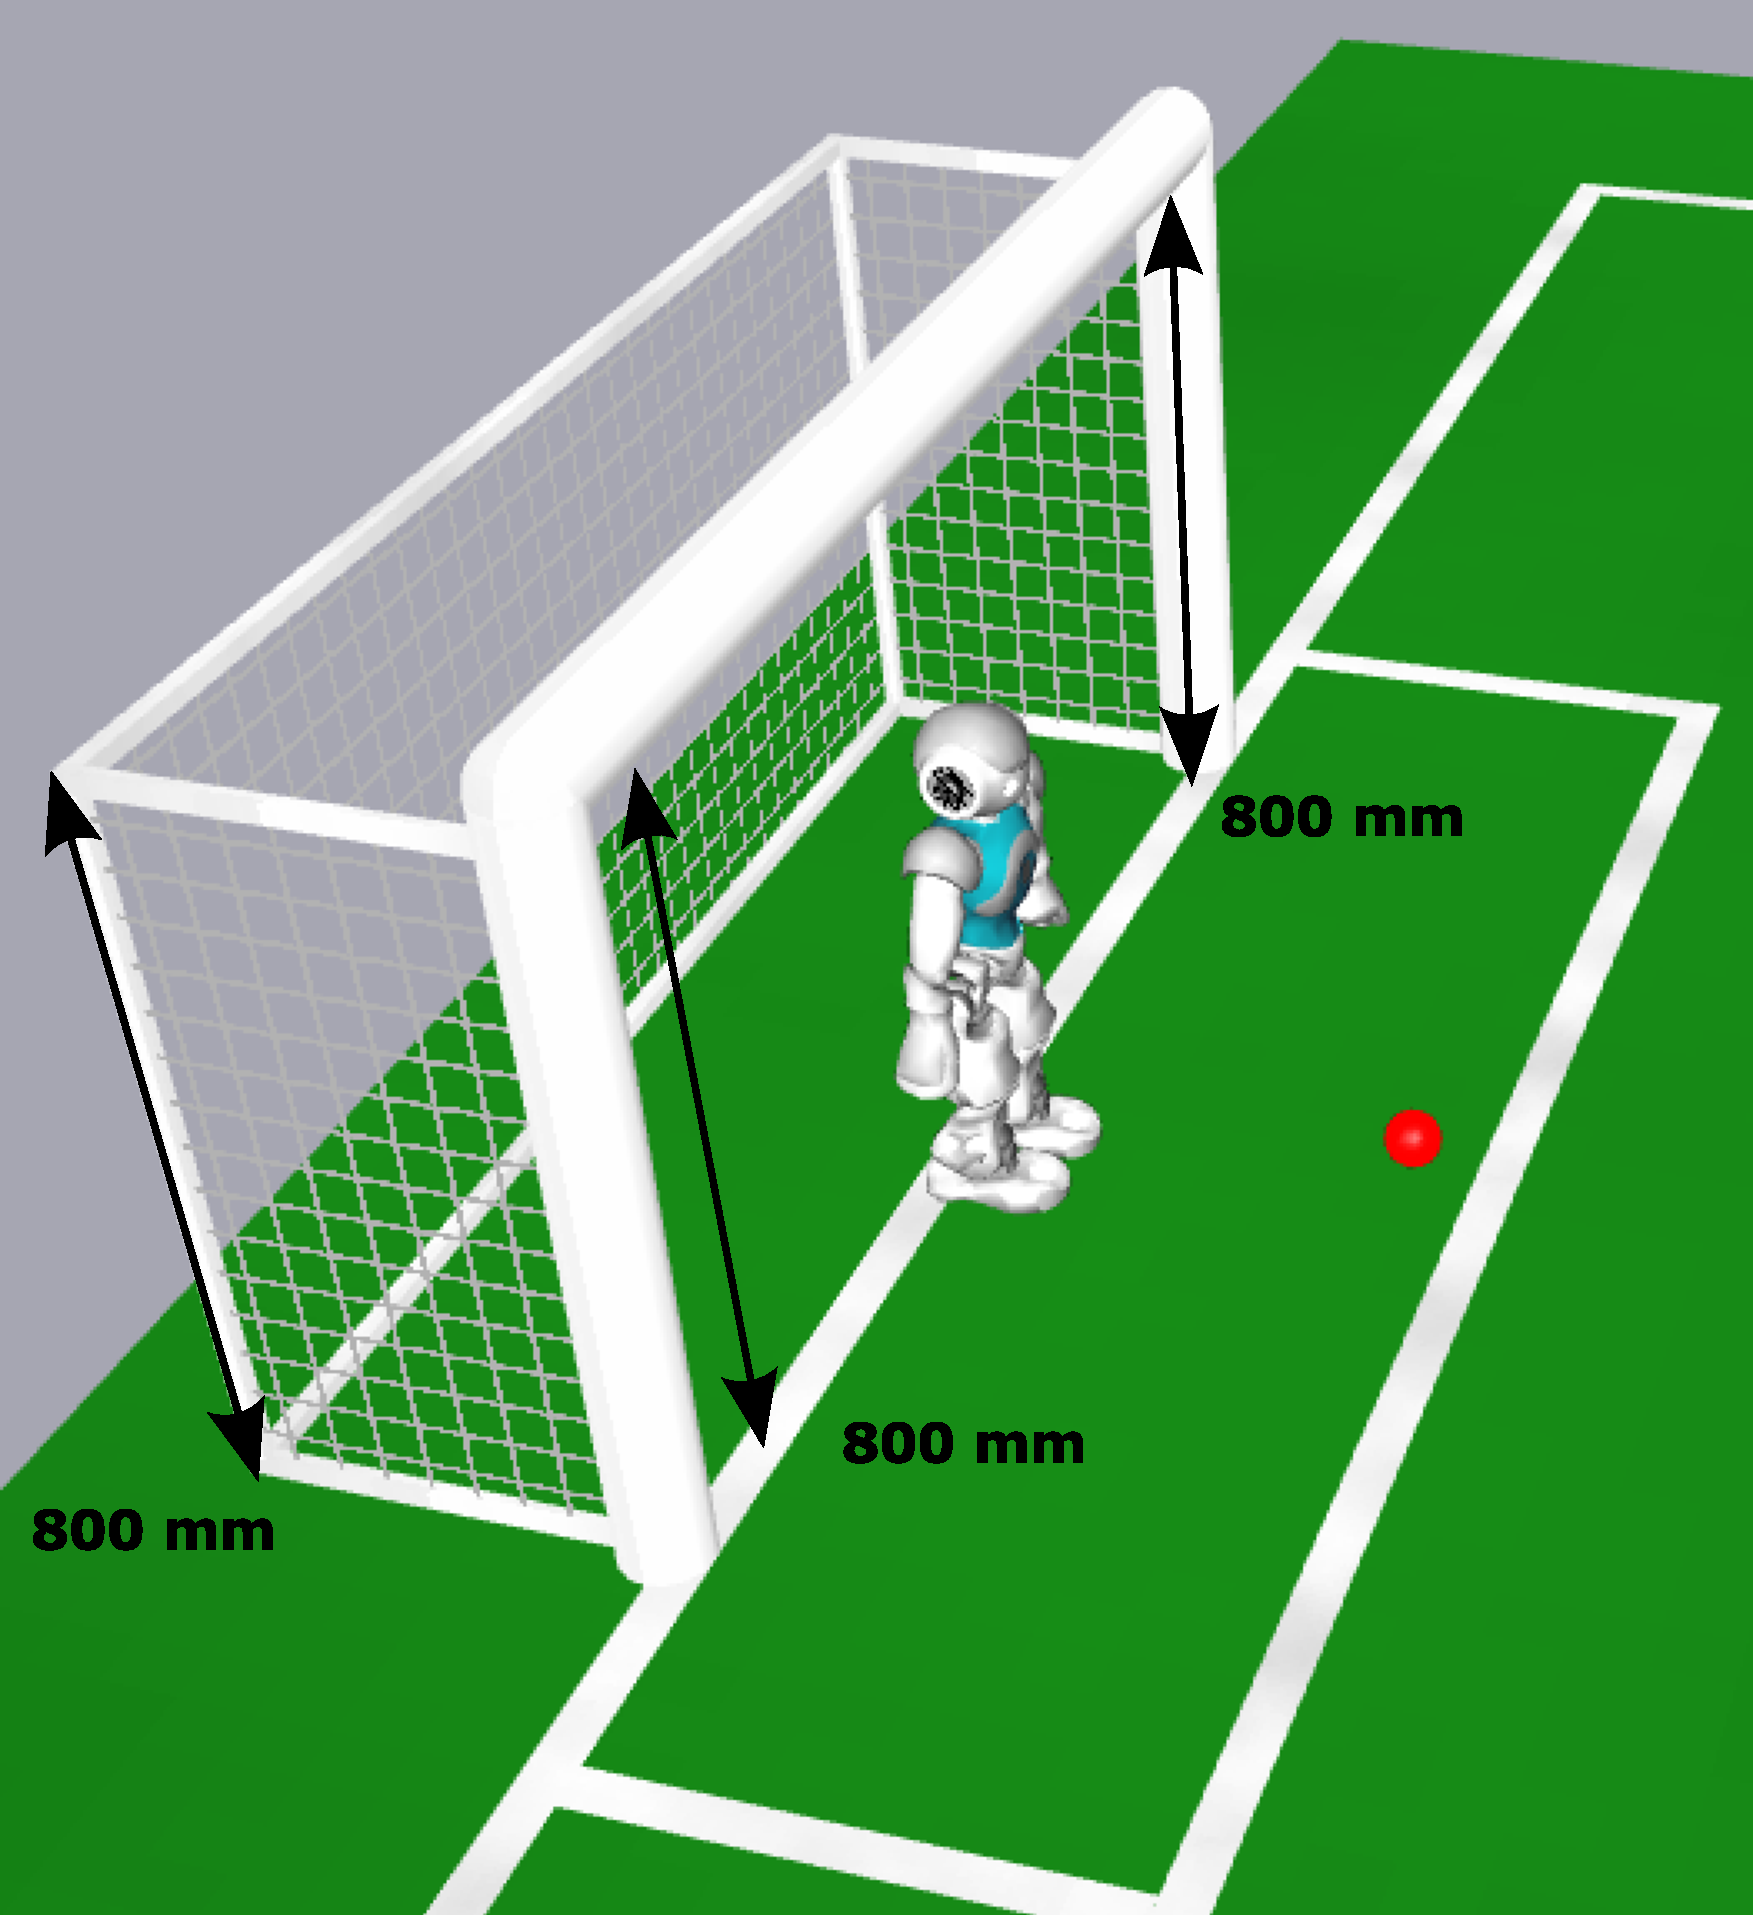
\includegraphics[width=1\columnwidth]{figs/goalDimensions3D.pdf}}%
\end{minipage}
\begin{minipage}[t]{0.49\columnwidth}
The goalposts and crossbar are made from 3 white cylinders with a diameter of \qty{100}{\milli\metre}.
The net:
\begin{itemize}
\item has a height of \qty{800}{\milli\metre}
\item is of white, gray or black color
\item is tightly supported via the support structure, in a way to minimize interference with the goalkeeper
\item has a weave with holes smaller than the ball diameter.
\end{itemize}
\end{minipage}
\caption{Appearance and dimensions of the goals.}
\label{fig:goal_appearance}
\end{center}
\end{figure}

\subsection{Field Colors}
\label{sec:field_colors}
The colors of the soccer field are as follow:

\begin{itemize}

\item The field (artificial turf) itself is green (color is not specified, but it should not be too dark).

\item The lines on the field are white, whether they are taped, spray painted or made from white artificial turf.

\item Goals~(\cf \cref{fig:goal_appearance}). The posts and top crossbar of both goals are white. The net and the support structure for the net are white, gray, or black.

\end{itemize}

\subsection{Lighting Conditions}
\label{sec:lightConditions}
The lighting conditions depend on the actual venue. SPL fields should be placed near or under windows where possible. Whether window lighting is used, ceiling lights should be provided as necessary to ensure that most of the field is never darker than 300 Lux (400 Lux preferred).

Lighting is not required to be even and hotspots may occur on the field. The lighting design (comprising both natural and artificial light sources) shall aim to limit the ratio between the brightest and darkest patches on the field to less than 10:1. In general, lighting irregularities, including changes that occur during the competition, are acceptable and will not be cause for delay.  Such irregularities may include sun streaming through windows, light bulbs turning off, light bulbs being replaced, etc.

\subsection{Venue Setup}
\label{sec:boundaries}
Fields may be located close to one another.  Barriers will not necessarily be constructed between adjacent fields to block the robots from seeing other fields, goals, or balls. However, barriers will be constructed to block sight between any fields that are not located at least three meters apart. Hence, for each side of a field that is adjacent to another field, either barriers will separate the fields or at least \qty{3}{\metre} will be between the carpet of adjacent fields.

\subsection{Ball}
\label{sec:ball}

The official ball is a soft foam ball with a black and white soccer ball print (see \cref{fig:ball}). They are \qty{100}{\milli\metre} in diameter and weight \qty{44}{\gram}. These balls are available by writing to \url{info@sportpaint.de} (in German or English) and asking to order the "pu schaumstoffball 10cm 100ss".  Each ball costs \euro{2.86} plus shipping, where shipping cost depends on the destination.

\begin{figure}[t]
  \centerline{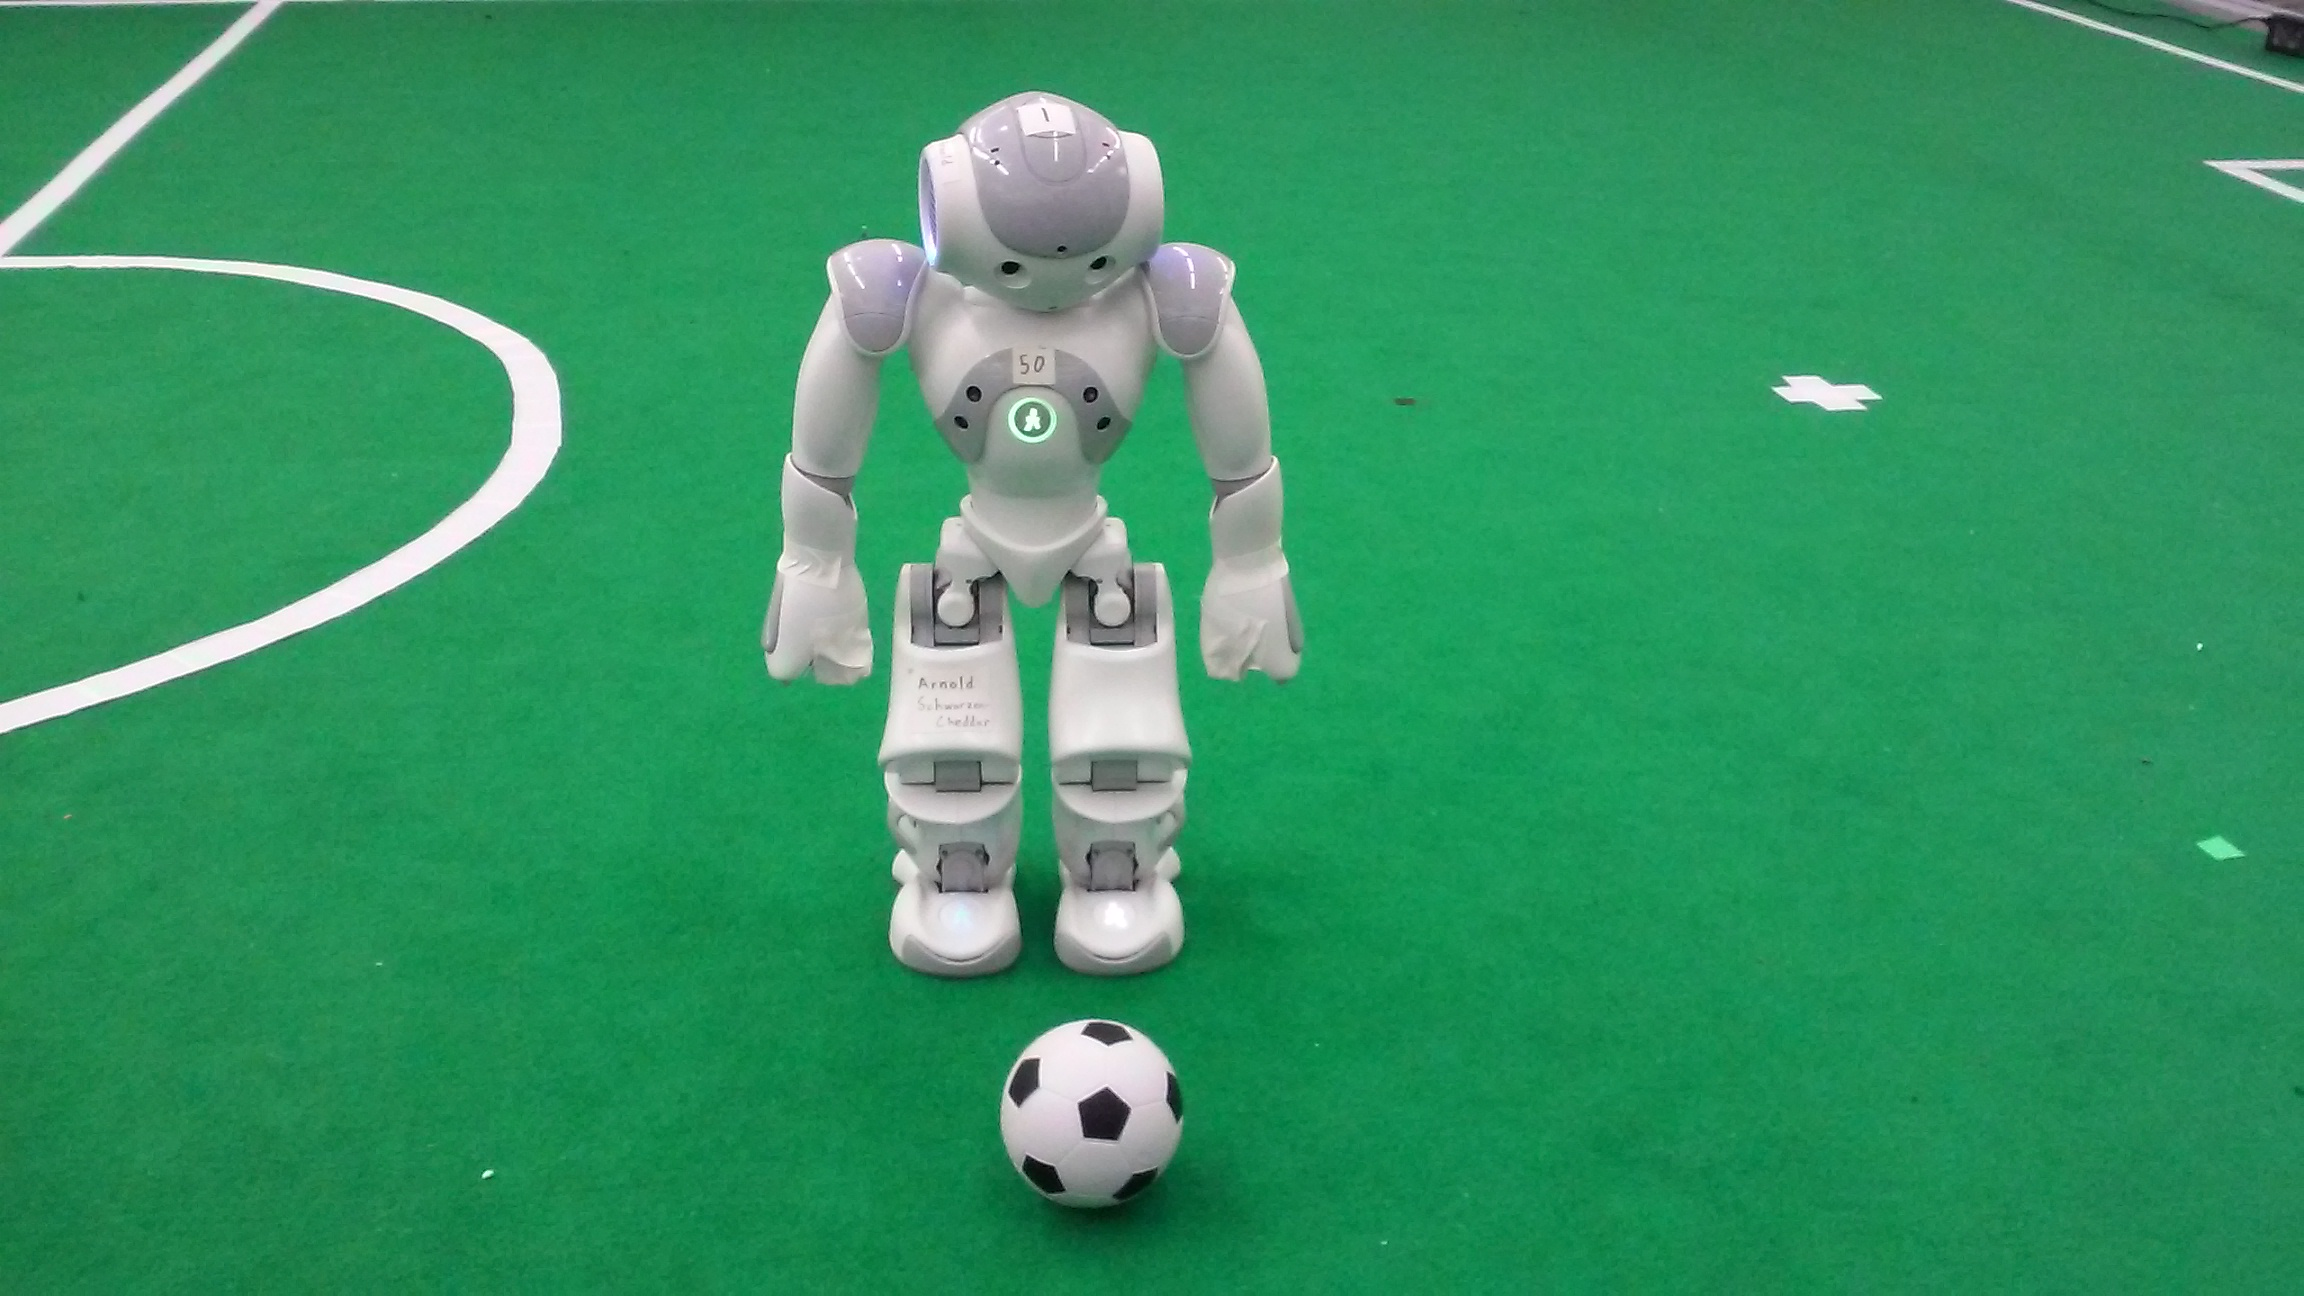
\includegraphics[height=0.28\columnwidth]{figs/robotWithBall2016.jpg}}
  \caption{A NAO and an official ball.}
  \label{fig:ball}
\end{figure}

\subsection{Definition of Inside and Outside}
\label{sec:inside_outside}

A line is always part of a region of the field.
This means, that \emph{inside/outside \textless region\textgreater} refers to the green area as well as the surrounding line.
Specifically:
\begin{itemize}
    \item The field boundary lines are part of the field
    \item The penalty area lines (and the end field line inside of the goal) are part of the penalty area
    \item The center circle lines are part of the center circle
\end{itemize}

The only \textit{exception} to this rule is the center field line, which does not form part of any half.
That is, a robot is \textit{outside} a half of the field if it is touching the center line.

\subsection{Streaming setup}
\label{sec:streaming_setup}

There are multiple use cases for a streaming setup: 
\begin{itemize}
	\item Stream all videos to RoboCup SPL Youtube channel to store them there
	\item Allow team members from remote to watch their robot's match
	\item Evaluate team's performance measures online from videos recording (Part of Technical Challenge 2022)
\end{itemize}
